\documentclass{article}

%%%%%%%%%%%%%%%%%%%%%%%%%%%%%%%%%%%%%%%%

\usepackage[utf8]{inputenc}

%%%%%%%%%%%%%%%%%%%%%%%%%%%%%%%%%%%%%%%%

\usepackage[dvipsnames]{xcolor} %may result in an error if you are using beamer with tikz. To go around it, include usenames and dvipsnames options when defining the document class, e.g. \documentclass[usenames,dvipsnames]{beamer}
\usepackage{tikz}
\usepackage{pgfplots}
\pgfplotsset{compat=1.5}

\usetikzlibrary{external}
\tikzexternalize
\tikzsetexternalprefix{tikzexternal/}

%%%%%%%%%%%%%%%%%%%%%%%%%%%%%%%%%%%%%%%%

\usepackage{amsmath,amsfonts,amssymb}
\renewcommand{\baselinestretch}{1.0}
\usepackage{graphicx}
\usepackage[colorlinks=true, allcolors=blue]{hyperref}
\usepackage{color, colortbl}
\usepackage{lscape}
\usepackage{enumitem}
%\usepackage{chngcntr}
%\counterwithin{figure}{section}
%\counterwithin{table}{section}
\usepackage{booktabs,caption}
\usepackage[flushleft]{threeparttable}

%%%%%%%%%%%%%%%%%%%%%%%%%%%%%%%%%%%%%%%%

\setlength{\parindent}{0pt}
\setlength{\parskip}{\medskipamount}

%%%%%%%%%%%%%%%%%%%%%%%%%%%%%%%%%%%%%%%%

\usepackage{newtxtext,newtxmath}

% Instead of the above, use this for arXiv:

%\usepackage{txfonts}
%\usepackage{textcomp}
%\usepackage{eurosym}
%\let\texteuro\euro

%%%%%%%%%%%%%%%%%%%%%%%%%%%%%%%%%%%%%%%%

\newcommand{\unit}[1]{\ensuremath{\mathrm{#1}}}
\newcommand{\micron}{\mbox{\textmu m}}
\renewcommand{\deg}{\mbox{deg}}
\newcommand{\sqdeg}{\mbox{$\deg^2$}}
\newcommand{\persqdeg}{\mbox{$\deg^{-2}$}}
\newcommand{\arcmin}{\mbox{arcmin}}
\newcommand{\sqarcmin}{\mbox{\arcmin$^2$}}
\newcommand{\persqarcmin}{\mbox{\arcmin$^{-2}$}}
\newcommand{\arcsec}{\mbox{arcsec}}
\newcommand{\sqarcsec}{\mbox{\arcsec$^2$}}
\newcommand{\persqarcsec}{\mbox{\arcsec$^{-2}$}}
\newcommand{\sqmm}{\mbox{mm$^2$}}
\newcommand{\deighty}{\ensuremath{d_{80}}}
\newcommand{\Hs}{\mbox{$H_\mathrm{s}$}}
\newcommand{\Ravg}{\mbox{$R_\mathrm{avg}$}}
\newcommand{\Tavg}{\mbox{$T_\mathrm{avg}$}}
\newcommand{\mm}{\mbox{mm}}

%%%%%%%%%%%%%%%%%%%%%%%%%%%%%%%%%%%%%%%%

\begin{document}

\pagestyle{empty}

\begin{center}

{\Large \bfseries DDRAGO and WOB Management Plan}

\vspace{2cm}

\begin{tabular}{ll}
Prepared by:&Alan M. Watson\\
&Rosalía Langarica\\
&Erica Lugo\\
Reviewed by:&Alan M. Watson\\
&Rosalía Langarica\\
Approved by:&Alan M. Watson\\
&Rosalía Langarica\\
%DDRAGO Reference:&Document 2\\
Reference:&COLIBRI-UNAM-PL-5\\
Version:&1.3\\
Date:&29 March 2022\\
\end{tabular}

\vspace{\fill}

DDOTI Project\\
Instituto de Astronom{\'\i}a\\
Universidad Nacional Aut\'onoma de M\'exico

\end{center}

\newpage

%%%%%%%%%%%%%%%%%%%%%%%%%%%%%%%%%%%%%%%%%

\pagestyle{plain}

\setcounter{tocdepth}{2}
\tableofcontents
\newpage

%\listoffigures
%\newpage

%\listoftables
%\newpage

%%%%%%%%%%%%%%%%%%%%%%%%%%%%%%%%%%%%%%%%%

\clearpage
\section*{Version History}

\begin{itemize}

\item Version 1.2 of 29 March 2022
\begin{itemize}
    \item Added the safety certification procedure in \S8.
\end{itemize}
\item Version 1.1 of 24 February 2022
\begin{itemize}
    \item Added the Ensenada team.
    \item Added graphic calendars.
    \item Added comments on risks.
\end{itemize}

\item Version 1.0 of 9 February 2022
\begin{itemize}
    \item Initial version based on the corresponding DDRAGUITO document.
\end{itemize}
\end{itemize}
\clearpage

%%%%%%%%%%%%%%%%%%%%%%%%%%%%%%%%%%%%%%%%%

\section{Introduction}

Before discussing the management plan, it is worth recounting some of the events in the project history that have lead us to our current position: that we first built the interim DDRAGUITO instrument with one optical channel  and now building the definitive DDRAGO instrument with two optical channels and provision for the WOB CAGIRE.

\subsection{History to Summer 2017}

In June 2016 the French and Mexican partners agreed on a conceptual design for the telescope and two instruments. The Mexican DDRAGO optical instrument would have two CCD channels and would pass infrared light to the French CAGIRE instrument. 

One unusual requirement on DDRAGO was that we were to deliver it (with at least one of the two channels) to the OHP at the start of 2019 in order to test the telescope with a full-field instrument. Recall that the telescope does not naturally deliver good images over the full 26 arcmin field and requires corrective optics.

Therefore, after the conceptional design review, the DDRAGO team worked continuously on the design. We had a successful PDR in February 2017, subsequently froze the telescope optical design so that ASTELCO and LAM could proceed to acquire and polish the telescope mirrors, and were aiming to have the CDR in November 2017. However, the path to CDR took some unexpected turns.

\subsection{Change to a SOFRADIR Detector}

In July 2017, the project elected to change the CAGIRE detector from a Teledyne H2RG device to a SOFRADIR device. This per se was not unexpected. However, the UNAM team was not aware that this would imply a change in the pixel size from 18 {\micron} to 15 {\micron}. This was apparently the result of a miscommunication between the Project Office at LAM and the UNAM team; the Project Office assures us that this change was mentioned during the PDR, but the UNAM team have no memory of hearing this information and we have not been able to find a written record. 

Regardless, the result was that our existing optical design for CAGIRE which gave a 26 arcmin field on a H2RG detector only gave a 21.7 arcmin field on a SOFRADIR detector. We investigated reducing the effective focal length of the infrared channel to compensate, but this came with an unacceptable cost in image quality. In August 2017 the Project Office, the CAGIRE team, and the DDRAGO team decided to maintain the same final focal length to preserve image quality and improve sampling at the cost of reducing the useful field by about 16\% from 26 arcmin diameter (225 square arcmin) to 21.7 arcmin square (215 square arcmin).

\subsection{Change of the Instrument Flange Distance}

In October 2017, only a few weeks before the planned DDRAGO CDR, we were informed that in order to accommodate the cable wrap, the instrument flange on the derotator would have to be moved outwards. 

The initial estimate was that it would have to be moved out by 40 mm. This was not compatible with the DDRAGO/CAGIRE optical design and DDRAGO mechanical design we have developed in the months from PDR.

LAM had already begun to polish M2, but immediately suspended this work pending a reconsideration of the implications of this mechanical change on the telescope optics. The UNAM team reoptimized the optical design for the telescope and DDRAGO (but not CAGIRE) and checked that the new optical design for DDRAGO could be accommodated mechanically. In early November, the UNAM team proposed an option that modified M2 but left M1 as before, and this was accepted by LAM.

The telescope-instrument interface was finally defined in summer of 2018.

\subsection{DDRAGUITO}

With the change in the instrument flange distance and the lack of a firm definition of the telescope-instrument interface, it was clear that we could not proceed to a CDR in November 2017 and would not be able to deliver the instrument as originally conceived for the start of 2019. 

Therefore, the UNAM proposed to split the instrument into an “interim instrument” called DDRAGUITO and a “definitive instrument” called DDRAGO. The interim instrument would be a simple structure containing only the unfolded blue channel, and was intended be delivered for tests at OHP in 2019. It would have no provision for the red or infrared channels. The definitive instrument would be delivered directly to the OAN in time for the arrival of the telescope.

When the telescope-instrument interface was finally defined in February 2018, the UNAM team reoptimized the DDRAGO and CAGIRE optics (the telescope optics had been frozen in November 2017), the telescope baffles, and the DDRAGO optomechanics, and designed from scratch the DDRAGUITO support struture.

In order to make purchases in time to deliver DDRAGUITO in 2019, we needed to have a CDR no later than May 2018. However, the time available to us was not enough to complete the redesign of the definitive instrument support structure. Therefore, in the CDR in May 2018, we presented the optical design of the telescope, DDRAGUITO, DDRAGO, and CAGIRE instrument, but in all other aspects (mechanics, AIV, control, and management) referred only to DDRAGUITO.

The direct costs of DDRAGUITO instrument are relatively small, since almost all of the components will be reused in the DDRAGO with the exception of the interim support structure (about US\$5,000). However, the indirect salary costs associated with first having to redesign the instrument to the new flange distance and then having to design and integrate are more significant. Worse, delivering DDRAGUITO has imposed a significant delay on the delivery of DDRAGO. On the other hand, it means that we will be testing the telescope at OHP with a much simpler instrument.

For the usual reasons, the delivery of DDRAGUITO was expected to be delayed from 2019 to the summer of 2020. However, at the start of 2020 the COVID-19 pandemic occurred, and this caused even more delays as initially we had no access to our laboratories and workships and then gained limited access. We finally shipped DDRAGUITO to OHP in March 2021.

DDRAGUITO has been verified optically at LAM after shipping and the control system and detector have been checked for aliveness at OHP. However, the OHP/LAM team have spent most of 2021 solving unexpected alignment problems with the telescope and, at the time of writing in late February 2022, DDRAGUITO has not yet been mounted on the telescope.

\subsection{DDRAGO and WOB}

After the delivery of DDRAGUITO, we turned our attention to finishing the design of DDRAGO and the WOB. This work involved designing the dichroic holders, the support structure, the WOB and its optomechanics for the lenses L5 to L11, the shutter, the focus stage, and the fold mirrors FM1 to FM3, and of course the interface to CAGIRE. We also worked closely with the UNAM infrastructure team, the project office at LAM/OHP, and our CAGIRE colleagues at IRAP to define the instrument handling procedures.

We intend to deliver DDRAGO with operational blue and red channels, a dummy WOB, a dummy CAGIRE cryostat, and a dummy CAGIRE close electronics and be ready for science operations in March or April 2023. IRAP will supply the dummy CAGIRE cryostat and close electonics. UNAM will supply the dummy WOB. The instrument will operate with the two CCD channels until the WOB and CAGIRE are completed.

We then intend to deliver the operational WOB for the middle of 2023 to the start of 2024. IRAP will supply the operational CAGIRE cryostat and close electronics. These components will be integrated at the telescope to give the final DDRAGO/CAGIRE combined instrument, with blue, red, and infrared channels.

\clearpage
\section{Work Packages}

The Mexican and French partners havce agreed that the French partners will be responsible for the telescope and infrared imager (CAGIRE) and the Mexican partners will be responsible for the optical imager (DDRAGO), infrastructure at the OAN, and operational support at the OAN.

\subsection{DDRAGO}

In June 2016 the French and Mexican partners agreed on a conceptual design for the telescope and two instruments. The UNAM immediately began to work on the design of DDRAGO in order to comply with the very tight schedule for delivery. 

\subsection{WOB}

Unfortunately, the funding from CNES to IRAP to develop CAGIRE was very limited in 2016. This created a technical problem, since the CAGIRE optics are deeply embedded in the common support structure. The solution to this was to agree that the UNAM would extend their work to cover the design of the warm optical bench (WOB) and IRAP would subsequently design the CAGIRE cryostat, filter wheel, close electronics, and control system.

In addition, the IRAP accepted the UNAM’s offer to fabricate the mechanical parts and to assemble and verify the WOB. The cost of the WOB optics was shared between the UNAM (the spherical lenses L5 to L7 and L9 to L11 and the fold mirrors FM1 to FM3) and LAM (the aspherical lens L8). The UNAM is supplying the focus stage for L7 and IRAP is supplying the WOB shutter and shutter controller.

\subsection{DDRAGUITO}

Following the late change in interface to the telescope, described above, the UNAM took on an additional work package to design, build, test, and deliver the interim instrument DDRAGUITO, consisting of only one unfolded optical channel.

Given the existence of this interim instrument, we refer to the full DDRAGO (with two optical channels and passing infrared light to CAGIRE) as the definitive instrument.

\clearpage
\section{Approach to Risk}

\subsection{DDRAGUITO as a Prototype}

We consider that we retired many of the risks in DDRAGO during the manufacture and AIV of DDRAGUITO. Of course, DDRAGUITO has not yet seen sky.

\subsection{Advanced Manufacture and Purchases}

If we waited until after the FDR to make all purchases and start all manufacture, we would add years to the delivery date. Furthermore, our funding would have expired. Therefore, we have been forced to make purchases and begin manufacture prior to the FDR. This obviously implies some risk. We have attempted to reduce this risk by concentrating our purchases and manufacturing in areas which have been previously reviewed. 

Our advanced purchases (see below) have been mainly in optics, filter wheels, and detectors. The main unreviewed items we have purchased are the focus stages, which cost about 10k€ in total.

Our advanced manufacturing has been in the optomechanics of L3, L4 (since the L1+L2 barrel will be reused unmodified from DDRAGUITO), and dichroics and corrector plate. The optomechanics of L1+L2 and L3 were reviewed for DDRAGUITO and those for L4 are very similar; we feel there is little risk here. The optomechanics for the dichroics and corrector plate are being reviewed for the first time in this review, so the risk is real. However, if we do need to  remanufacture these as a result of this review, the cost is small, since they are being manufactured in-house.

\subsection{Availability of Materials}

We still need to make purchases of certain specialized materials (engineering plastics). These are proving to be difficult apparently because of a global shortage. We will work on this as soon as the FDR documentation is delivered.

\clearpage
\section{Purchases and Budget}

We have made all major purchases for DDRAGO and WOB, including:

\begin{itemize}
    \item The blue CCD system (delivered and integrated in DDRAGUITO).
    \item The red CCD system, including spare hoses and cables for installation at the telescope (ordered in fall 2021 with delivery expected in June 2022).
    \item The three filter wheel (two operational and one spare, all delivered, and one integrated in DDRAGUITO).
    \item The 10 filters ($g$, $r$, $i$, $z$, $y$, $gri$, $yz$, $B$, and three uncoated, parfocal fused silica substrates, all delivered and sent with DDRAGUITO).
    \item The lenses L1 and L2 (delivered and integrated in DDRAGUITO).
    \item The lenses L3B (a replacement for the damaged L3 integrated in DDRAGUITO) and L4 (both delivered).
    \item The dichroics D1 and D2 and the corrector plate CP (ordered in 2020 with delivery expected in 2022).
    \item The lenses L5 to L7 and L9 to L11 (ordered in fall 2020 with delivery expected in spring 2022)
    \item The fold mirrors FM1 to FM3 (order in fall 2021 for delivery in spring 2022).
    \item The two focus stages with controllers (one operational and one spare, both delivered).
    \item Sufficient Alumold for the optomechanics and the support structure.
    \item Advanced payment for the fabrication of the support structure plates in an external workshop.
\end{itemize}

In addition, the following items are being purchased by our partners:

\begin{itemize}
    \item L8 (to be ordered by LAM in spring 2022)
    \item The two WOB shutters and controllers (ordered by IRAP).
\end{itemize}

In the case of L5 to L11, D1, D2, and CP, the long delay between the order and delivery is due our need to purchase these in advance before the specifications were finalized. We essentially paid the vendors in 2020 on the basic of quotations for draft specifications and only confirmed the final specifications in 2021.

The outstanding costs for 2022 are: the parts for the instrument cart, anodizing; paint; minor materials such as nylon and mylar for the dichroic holders; fasteners; and shipping. We estimate a cost of about 25k€ and will use internal UNAM funds.

\clearpage
\section{Work Calendar}

The scope of our work calendar for the DDRAGO interim instrument is:

\begin{itemize}
\item Return of DDRAGUITO from OHP after testing for reuse of L1+L2, the L3 optomechanics, the blue detector and filter wheel and its optomechanics, and the control system.
\item Fabrication, assembly, and verification of DDRAGO, the WOB dummy, and the instrument cart.
\item Delivery to OAN.
\item Integration of the CAGIRE dummy cryostat and close electronics at OAN.
\item Installation and commissioning of DDRAGO with the dummies at OAN.
\item Fabrication, assembly, and verification of the WOB.
\item Integration of the WOB at OAN, along with the CAGIRE cryostat and close electronics supplied by IRAF.
\item Support for the CAGIRE commissioning carried out by IRAP.
\item Ten years of service on the telescope.
\end{itemize}

We have estimated the effort required for the fabrication of DDRAGO. We can convert this to a real-time estimate under two assumptions. 

The first is that the various manufacturing processes (conventional, CNC, laser/cutter, and metrology) can occur in parallel, since they involve different people. However, anodization, painting, and integration must occur in series. We assume that system-level verification can occur in parallel with the manufacture of the instrument cart.

The second is whether we continue with our current health regulations, with only one person working at a time in our workshop, or we return to normal working, with two persons working at a time in the workshop. These two options will be indicated by a range.

\begin{figure}
    \centering
    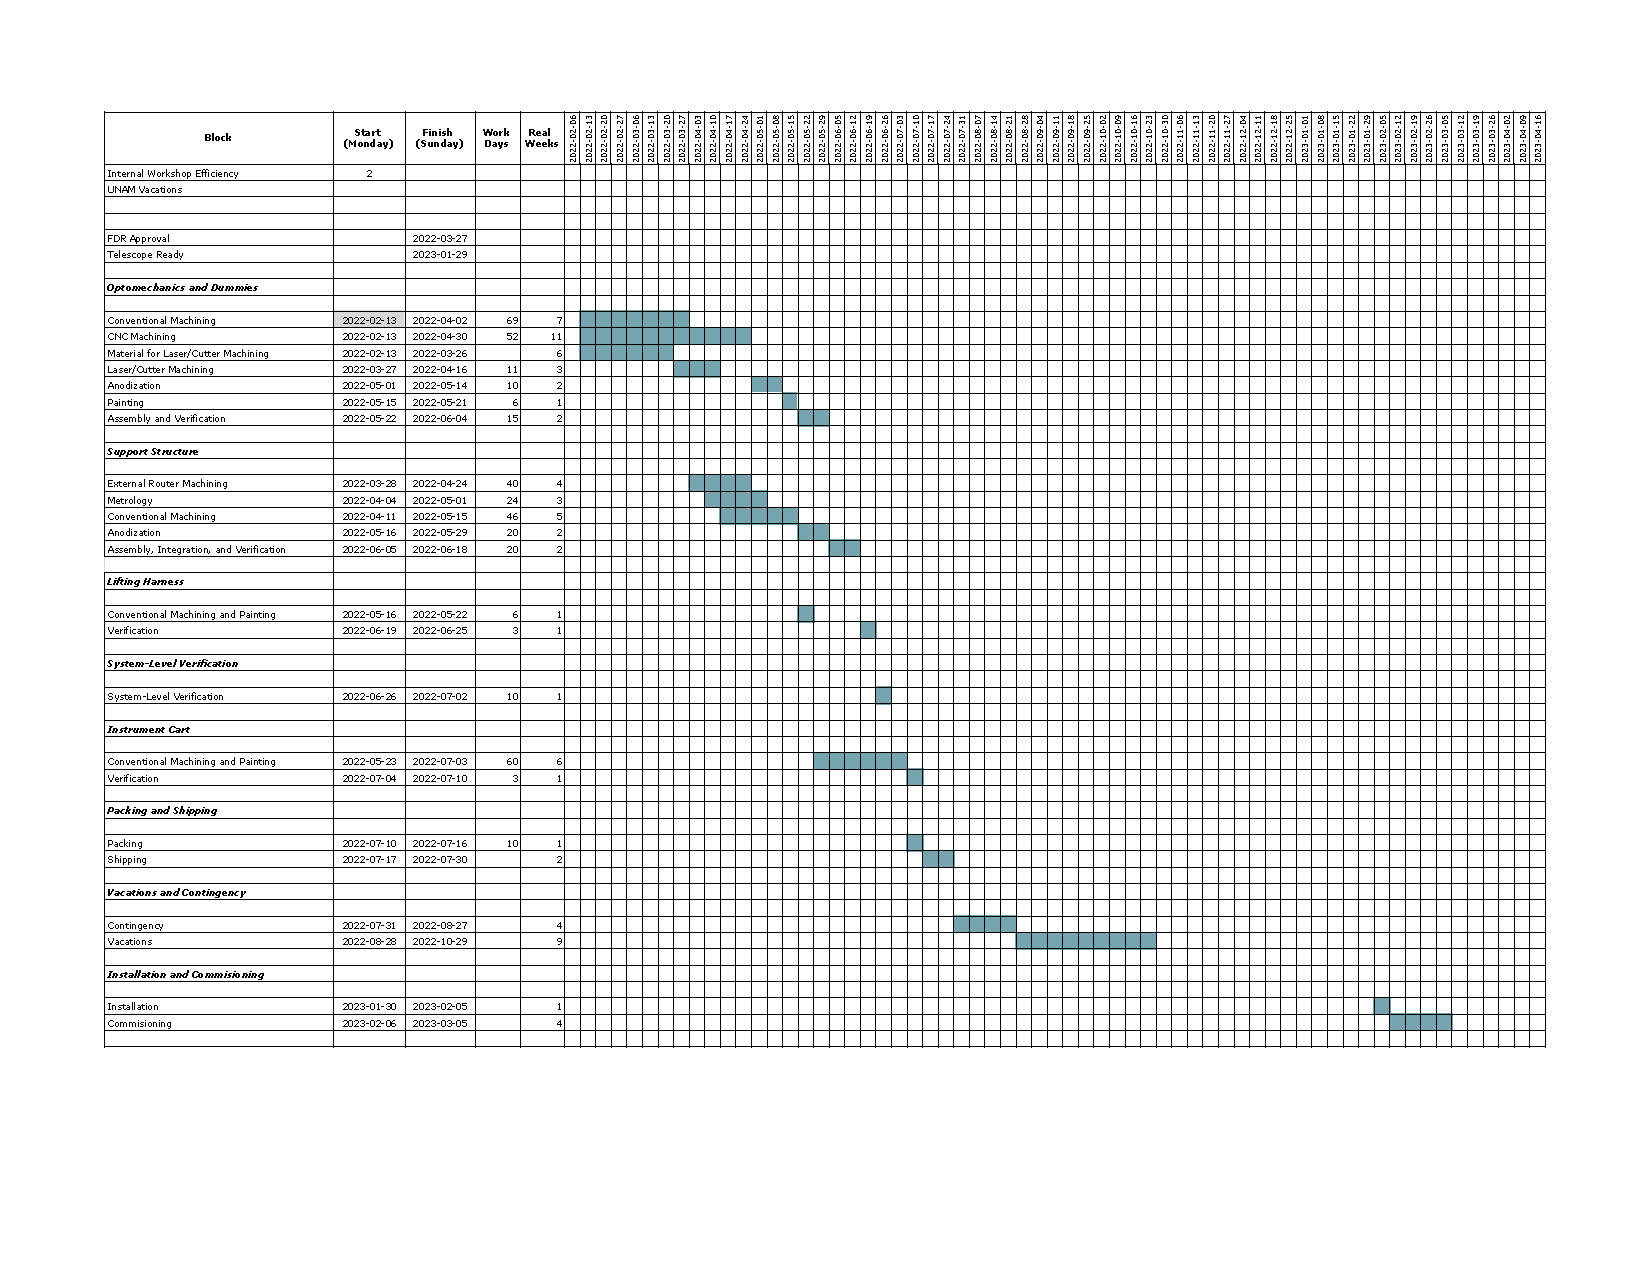
\includegraphics[angle=90,width=1.0\textwidth]{figures/calendar-optimistic.pdf}
    \caption{Optimistic calendar for the delivery of DDRAGO}
    \label{figure:calendar-optimistic}
\end{figure}

\begin{figure}
    \centering
    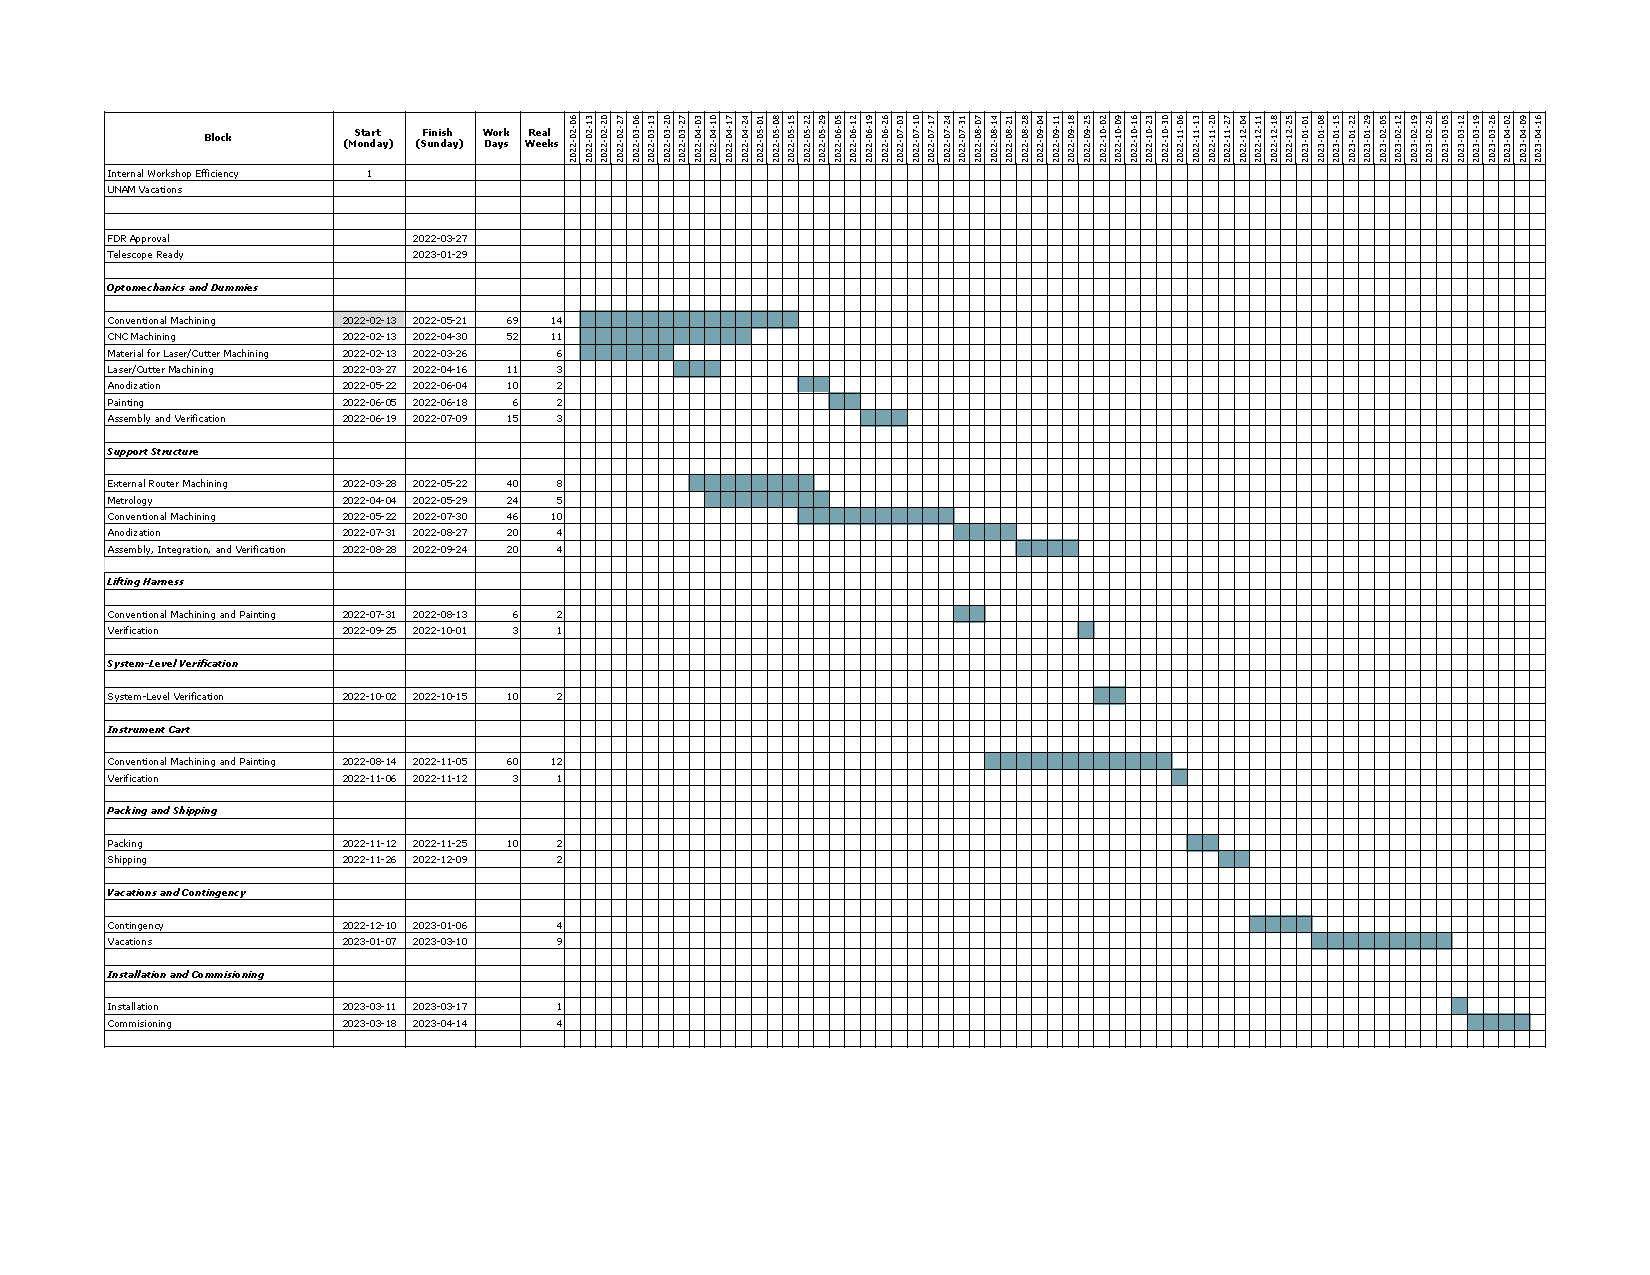
\includegraphics[angle=90,width=1.0\textwidth]{figures/calendar-pessimistic.pdf}
    \caption{Pessimistic calendar for the delivery of DDRAGO}
    \label{figure:calendar-pessimistic}
\end{figure}

The optimistic calendar, assuming two personas can work in the workshop, is shown in Figure~\ref{figure:calendar-optimistic}. It has the instrument being delivered to the OAN at the end of October 2022. Installation and commissioning will then have to wait for the telescope, which we assume will be ready for DDRAGO at the end of January 2023. Commissioning then takes a month and the instrument is ready for science at the start of March 2023.

The pessimistic calendar, assuming only one person can work in the workshop, is shown in Figure~\ref{figure:calendar-pessimistic}. This has the instrument being delivered to the OAN at the middle of March 2023 and being ready for science in the middle of April 2023.

The calendars show the major processes. We are monitoring progress within each process on a piece-by-piece basis and update the calendar every week (except for weeks when we are overwhelmed preparing documentation for the FDR).

The calendar for the WOB is almost completely dominated by conventional manufacture. Essentially, it requires 204 person-days of conventional manufacture followed by about 40 days of anodization, repeat metrology, integration and verification. Delivering the WOB with thus take 8 to 15 months, depending on whether one or two persons can work in the workshop, and can start as soon as the conventional manufacture of DDRAGO is completed (August 2022 to November 2022). Thus, in the optimistic case we would expect to deliver the WOB in May 2023 and in the pessimistic case at the start of 2024.

%The calendar for the WOB is:
%
%\begin{itemize}
%    \item Manufacturing:
%    \begin{itemize}
%        \item Conventional: 204d
%        \item Outside machining: 1d
%        \item Laser/Cutter:21d
%        \item Metrology: 25d
%        \item Subtotal: 102d--204d
%    \end{itemize}
%    \item Anodization: 10d
%    \item Painting: 2d--4d
%    \item Integration and Verification: 18d
%    \item Subtotal: 132d--236d
%    \item Contingency at 10\%: 13d--24d
%    \item TOTAL: 135d--260d
%\end{itemize}

\section{Technical Team}

The UNAM team for DDRAGO/WOB consists of:
\begin{itemize}
\item Alan Watson. DDRAGO PI. Management. Control. Software.
\item William Lee. COLIBRÍ Co-PI. Management.
\item Rosalía Langarica. Project manager. Mechanics (optomechanical design and integration).
\item Silvio Tinoco. Mechanics (optomechanical design, fabrication, metrology, and integration)
\item Alejandro Farah. Mechanics (structural design, fabrication, metrology, and integration).
\item Jaime Díaz. Mechanics (fabrication and metrology).
\item Benito Serralde. Mechanical (fabrication).
\item Diego Orozco. Mechanical (fabrication).
\item Salvador Cuevas. Optics (design, assembly, and integration).
\item Jorge Fuentes. Optics (design, assembly and integration).
\item Oscar Chapa. Optics (characterization).
\item Luis Carlos Álvarez. Optics (characterization).
\item Fernando Ángeles. Control. Electronics.
\item Silvio Tinoco. Mechanical (fabrication and metrology).
\end{itemize}

In addition, we work with members of the COLIBRÍ Infrastructure team in Ensenada on instrument handling issues:
\begin{itemize}
\item Alan Watson. Infrastructure PI. Management.
\item William Lee. COLIBRÍ Co-PI. Management.
\item Erica Lugo. Project manager.
\item Liliana Figueroa. Civil engineering.
\item María Herlinda Pedrayes. Mechanical engineering.
\item Eduardo López. Mechanical engineering and mirror coating.
\item Edgar Cadena. Electrical and electronic engineering.
\item José Luis Ochoa. Electrical and electronic engineering.
\end{itemize}




\clearpage
\section{Maintenance Plan}

We will write the maintenance manual during verification and commissioning.

We are planning to have spares and documentation on site so that local staff can carry  the following corrective maintenance with only remote support from the DDRAGO team:

\begin{itemize}
\item Powering the instrument off.
\item Powering the instrument on.
\item Diagnosis of the CCD, filter wheel, and environmental sensors.
\item Switching to the Spare CCD PC or Spare Control PC.
\item Replacing a failed Ethernet switch
\item Replacing a failed iBootBar
\item Using the spare cables.
\item Replacing a CCD with its dummy and vice versa.
\item Installing the spare filter wheel.
\item Installing the spare shutter.
\item Replacing failed 1-Wire sensors.
\end{itemize}

Some of these tasks may also require remote intervention by the DDRAGO team to reconfigure the control system or perform remote configuration of hardware. However, our aim is that they will not require the DDRAGO team to travel to OAN.

We will supply the following spares on site:
\begin{itemize}
\item Spare filter wheel
\item Spare 1-wire sensors
\item Spare CCD and Control PCs
\item Spare iBootBar
\item Spare Ethernet switch
\item Spares for every item in the electronics cabinet
\item Spare cables
\item PT-30 gas
\end{itemize}

\clearpage
\section{Safety Certification}

The OAN will supervise the certification of the instrument under the appropriate Mexican safety regulations (“Normas Oficiales Mexicanas” applicable to the instalation, operation, and mantenance of the instrument. The process will include a review of the safety measures detailed in the manuals for the instrument and its associated equipment. We consider the following regulations to be applicable:

\begin{itemize}
    \item NOM-001-STPS-2008 Edificios, locales e instalaciones
    \item NOM-009-STPS-2011 Trabajos en altura
    \item NOM-029-STPS-2011 Mantenimiento de instalaciones eléctricas
    \item NOM-004-STPS-1999 Sistemas de protección y dispositivos de seguridad en la maquinaria y equipo que se utilice en los centros de trabajo
    \item Normas de Salud (Personal)
    \item NOM-025-STPS-2008 Iluminación
    \item NOM-036-STPS-2018 Factores de riesgo ergonómico. Parte 1: Manejo manual de cargas
    \item NOM-001-SEDE-2005. Instalaciones eléctricas (utilización)
\end{itemize}

The supervision will formally start with the delivery of the instrument to OAN and will continue during the life of the instrument.

Each month, the OAN reports on the certification of the equipment under its control, which will include DDRAGO, to the following authorities:

\begin{itemize}
    \item Comisión Especial de Seguridad (UNAM)
    \item Protección Civil (UNAM)
    \item Protección Civil (Municipal)
    \item Protección Civil (State)
    \item Comisión Federal de Electricidad (Federal)
\end{itemize}

\clearpage
\section{Insurance}

DDRAGO will be owned by the UNAM. As such, it will be self-insured both in transit and at the telescope.

\end{document}

